\documentclass[a4paper,12pt]{article}
\usepackage{combelow}
\usepackage{graphicx}
\usepackage{titlepic}
\usepackage[T1]{fontenc}

\graphicspath{{./images/}}

\makeatletter
\renewcommand{\fnum@figure}{\textbf {Fig.} \thefigure}
\renewcommand\tablename{\textbf{Tabel}}

\makeatother


\begin{document}
\begin{titlepage}
\centering
    \vspace*{\fill}

    \Huge\bfseries
    Caiet de practica

    \vspace*{1.5cm}
	
\includegraphics[width=8cm]{university_logo.png}
	\vspace*{0.5cm}

    \large {Constantin Miron Ma\cb{s}ca\\ 
    Universitatea Tehnic{\u a} Cluj-Napoca\\
    Prof. Radu-R{\u a}zvan Slavescu\\}
	
	\vspace*{1.5cm}
	\normalsize{28.06.2017 - 4.09.2017}

    \vspace*{\fill}
    
    \end{titlepage}

\tableofcontents{}
\clearpage

\section{Sinteza Activi{\cb t}{\u a}tilor}

 Continuand dezvoltarea proiectului de semestru din cadrul cursului de Sisteme Inteligente, s-a incercat obtinerea unui sistem care poate extrage informatii relevante din descrierea in limbaj natural a dozajului unui medicament. 
 
 Utilizand tehnici de procesare a limbajului natural, s-au studiat si aplicat diversi algoritmi si metode pentru a putea realiza un astfel de sistem. Limbajul de programare utilizat predominant este python datorita implementarilor bine documentate ale multor algoritmi de Machine Learning si NLP.
 
 Printre metodele/algoritmii cu care s-a experimentat se numara: clustering folosind tree-distance, affinity propagation, k-means, agglomerative clustering, MDS, chunking, conditional random fields, etc. 

\clearpage
\section{Activita{\cb t}i desf{\u a}{\cb s}urate}

\subsection{Proiect ini{\cb t}ial}

Activitatea a avut ca baza proiectul de semestru pentru cursul de Sisteme Inteligente. Acest proiect are scopul de a crea un sistem de extragere de informatii din text natural, mai precis din descrierea dozajului un medicament. Informatiile de extras sunt cantitatea dozajului, unitatea de masura, perioada, frecventa de dozare etc.

S-a incercat o abordare de clusterizare pe baza distantei dintre arbori. Textul care descria dozajul medicamentului era parsat utilizand suita Stanford NLP si transformat intr-un arbore.

  \begin{figure}[h]
 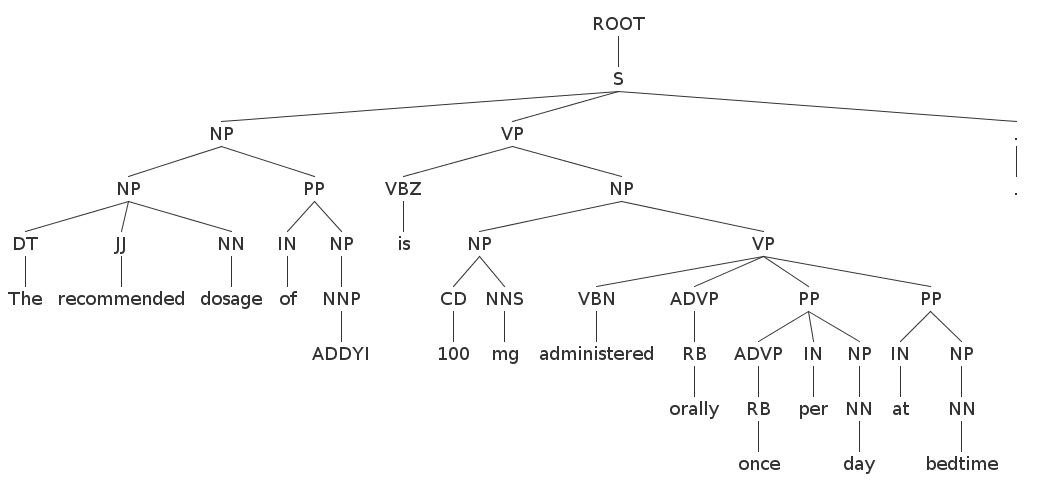
\includegraphics[width=12cm]{Tree.png}
 \caption{Structura de arbore pentru propozitia: "The recommended dosage of ADDYI is 100 mg administered orally once per day at bedtime."}
 \end{figure}

Dupa ce s-a obtinut un set de date de mai mult de 1000 de propozitii, s-a calculat o matricea de distante dintre arborii asociati. 

Distanta dintre doi copaci (Tree-edit distance) se calculeaza in functie de numarul de modificari (redenumire, stergere sau adaugare) care trebuiesc facute asupra nodurilor unui arbore pentru ca acesta sa fie transformat in al doilea.

Utilizand algoritmul Agglomerative Clustering s-a realizat clusterizarea arborilor pe baza matricei de distanta in speranta de a ii grupa in functie de modul de exprimare al dozajului.

Realizand un numar mai mare de matrici de distante pentru 150,200..1000 de arbori s-a realizat graficul din figura 2.

Se poate observa o tendinta logaritmica in grafic, ceea ce indica spre o realizare a problemei utilizand abordarea utilizata.

\begin{figure}[h]
 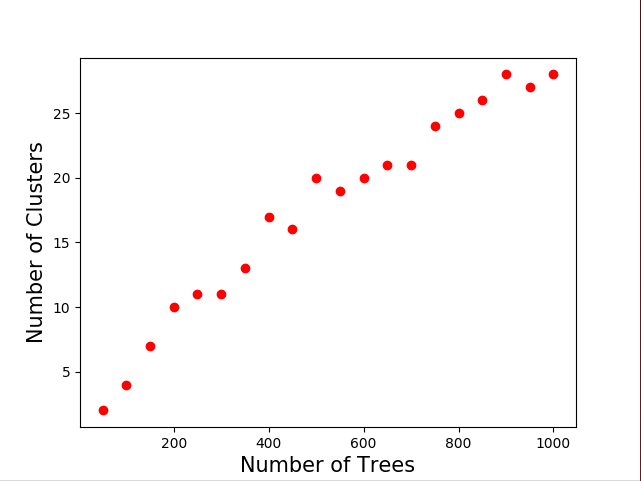
\includegraphics[width=12cm]{Result.png}
 \caption{Relatia dintre numarul de arbori si numarul de grupuri in care acestia pot fi incadrati}
 \end{figure}
 
 
\subsection{Continuarea abordarii bazate pe clustering}

Dupa reorganizari ale setului de date, corecturi ale fisierelor corupte sau care nu contin date relevante si schimbari de format ale matricilor de distanta, s-au studiat alti algoritmi de clusterizare:
\begin{itemize}
\item hierarchical clustering
\item k-means
\end{itemize}

Dintre acestia, algoritmul hierarchical clustering a prezentat cel mai mare interes datorita posibilitatii de realizare a unei dendrograme cu clusterele obtinute. 

In urma clusteringului folosind algoritmul ierarhic s-a obtinut o dendrograma, o sectiune a acesteia fiind prezentata in figura 3.
\clearpage
\begin{figure}[h]
\centering
 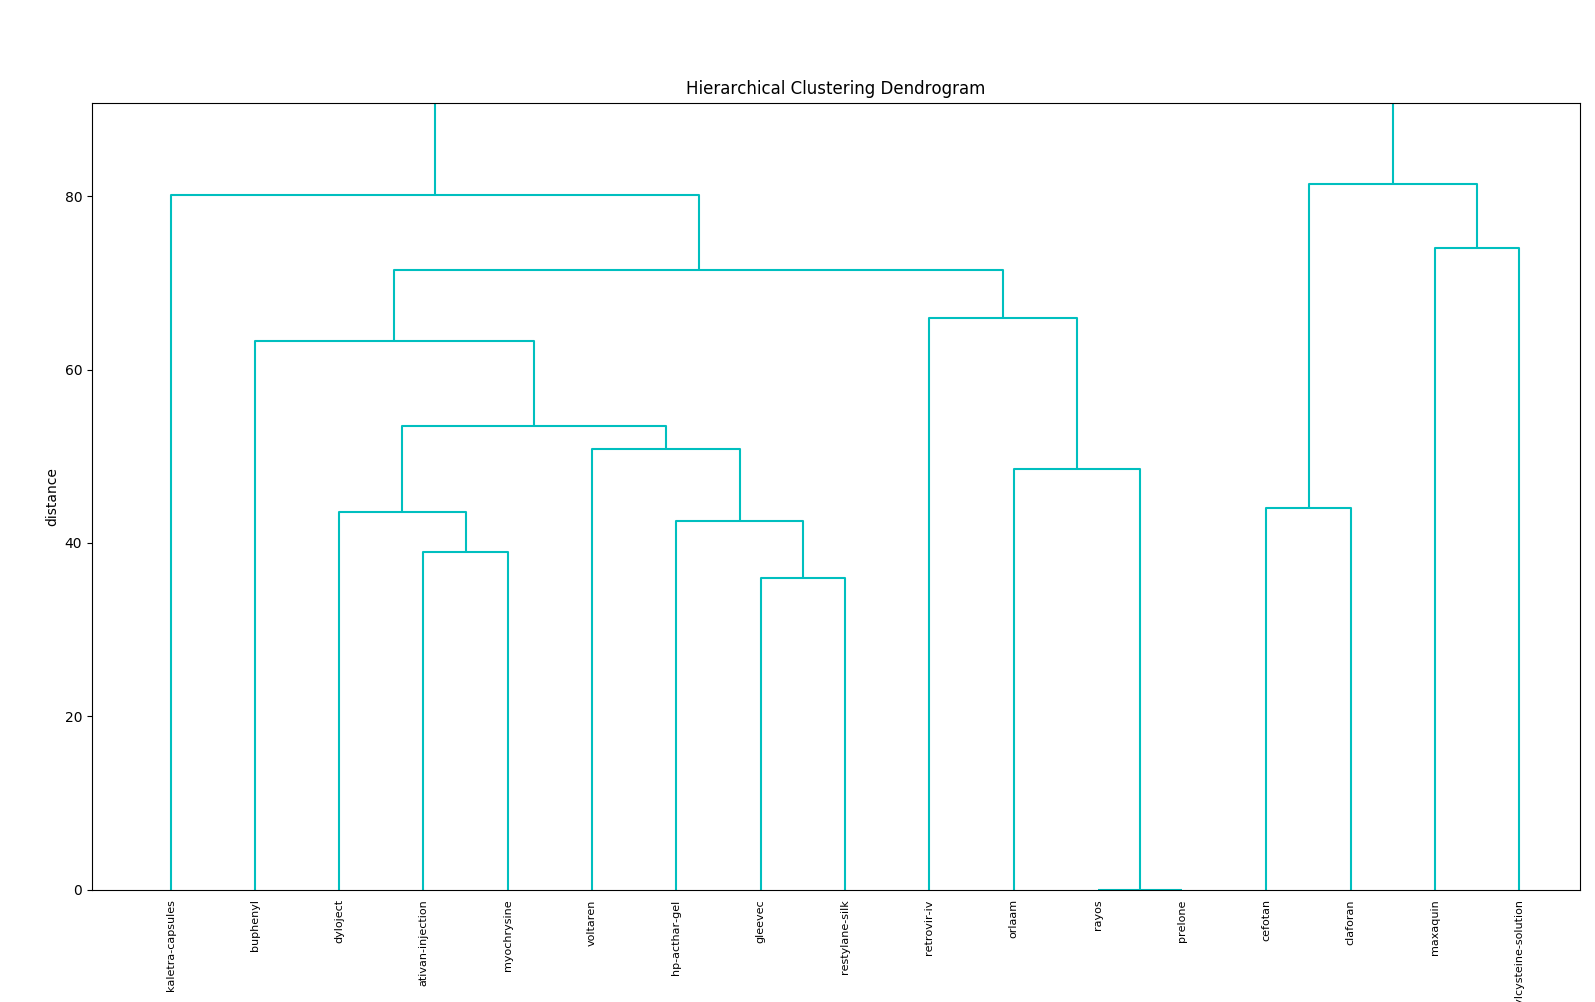
\includegraphics[width=16cm]{Hierarchical.png}
 \caption{Sectiune a dendrogramei realizate utilizand Hierarchical Clustering}
 \end{figure}

Interpretand dendrograma am putut observa ca distantele dintre clustere erau foarte apropiate, deci nu se obtineau clustere care sa fie foarte diferite - un prim indiciu ca abordarea de a clusteriza direct arborii nu poate oferii rezultate.

Alta abordare de vizualizare a setului de date a fost realizata utilizand un algoritm de scalare multidimensionala (MDS - multidimensional scaling). Luand ca si input matricea de distante, se calculeaza coordonatele pentru punctele care reprezinta arborii astfel incat aceste puncte sa fie la distantele indicate in matrice. 

Aceasta metoda de vizualizare, indiferent de numarul dimensiunilor in care au fost proiectate punctele, nu a oferit vreun indiciu spre o posibila grupare a arborilor.

Clusterizarea cu k-Means a fost efectuata utilizand coordonatele rezultate in urma scalarii multi dimensionale ca si input pentru algoritm. Utilizarea algoritmului prezenta urmatoarele probleme:
\begin{itemize}
\item cum se alege numarul optim de clustere dorit? (elbow method)
\item in cate dimensiuni sa se efectueze MDS? (curse of dimensionality)
\end{itemize}


\clearpage
\begin{figure}[h]
\centering
 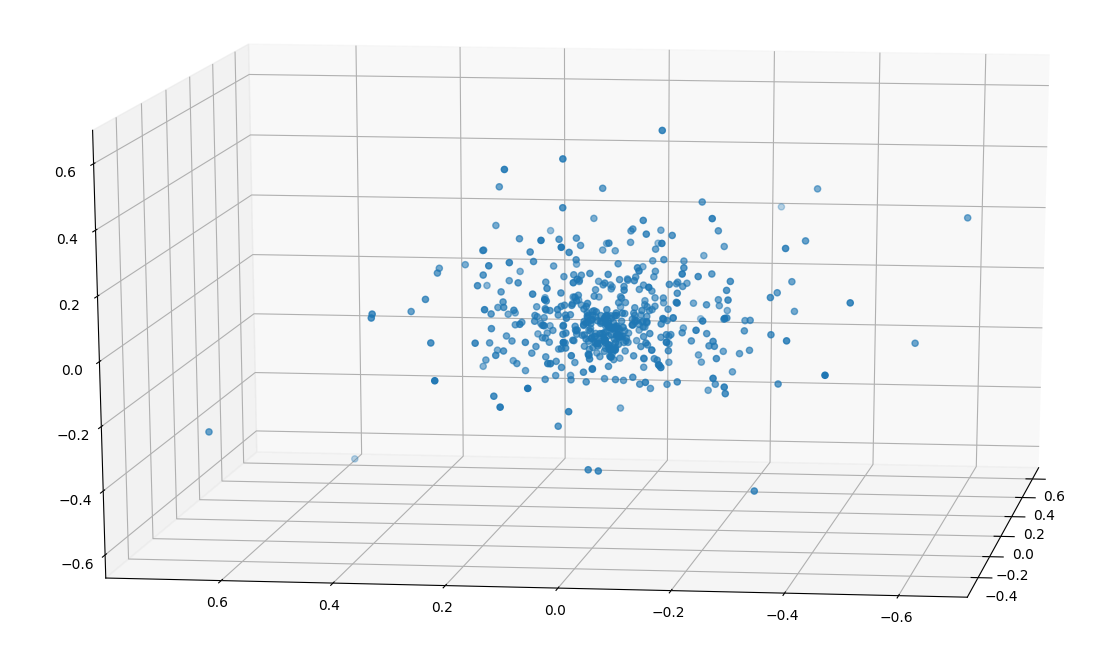
\includegraphics[width=16cm]{mds.png}
 \caption{Multidimensional scale 3D pentru matrice distanta de 500 de arbori}
 \end{figure}
 
 In timpul experimentarii cu acesti algoritmi s-au realizat diverse functionalitati pentru a usura manipularea, vizualizarea si accesul la setul de date.
 
 Concluzia la care s-a ajuns dupa aceste diverse abordari este ca o incercare de a clusteriza arborii nu poate fi utila. Arborii nu se grupau dupa modul de exprimare, cum ar fi fost ideal, in schimb lungimea propozitiilor fiind prioritara.
 \clearpage
 
 \subsection{Regenerarea setului de date}
 Pentru inceput, tot setul de date a fost refacut. Implementand o aplicatie care sa asiste la acest proces, am selectat manual cate o propozitie care continea dozajul efectiv dintr-un paragraf care descria detaliat dozajul unui medicament. 500 astfel de propozitii au fost obtinute, procesand 1000 de paragrafe. Acest nou set de date este corect si mai divers in exprimare fata de celalalt.
 
 Procesul prin care a trecut setul initial de date a fost repetat si pentru acesta. Pasii au fost urmatorii:
 \begin{itemize}
 \item generare parse-tree pe baza propozitiei
 \item reformatarea arborilor pentru a putea fi calculata distanta dintre arbori
 \item generarea matricei de distante
 \item generarea unei imagini pentru fiecare arbore pentru vizualizare
 \end{itemize}
 
 Clusterizarea noului set de date nu a oferit rezultate mai bune, deci am procedat spre idei noi de a obtine rezultatele dorite. 
 
 \subsection{Chunking}
 Am studiat procesul de NE(named entity) recognition urmarind cartea NLTK - o platforma de procesare de limbaj natural implementata in python.
 De asemenea, am realizat cateva expresii regulate pentru chunking. 
 
 \textbf{ DOSAGE: \{<VBZ><CD><NN>\}}

Chunking functioneaza pe baza unui regex care opereaza la nivel gramatical. In exemplul simplu de mai sus, partile componente ale regexului sunt urmatoarele:
\begin{itemize}
\item "DOSAGE": eticheta chunk-ului
\item VBZ: Verb, persoana a 3-a, singular, prezent
\item CD: numar
\item NN: substantiv singular
\end{itemize}

Desigur, o abordare bazata pe regex nu este una eficienta, exhaustiva sau poate chiar realizabila, dar aceasta tehnica poate fi de ajutor in viitor, dupa mai multa preprocesare.

\subsection{Conditional Random Fields}

Conditional random fields, sau CRF sunt algoritmi de tip classifier care functioneaza pe baza unui sistem probabilistic. Cea mai relevanta caracteristica a unei astfel de metode este natura secventiala a modelului, adica se ia in considerare contextul. Procesand limbaj natural, un astfel de algoritm este potrivit.

S-a utilizat crfSuite, implementat in python pentru testarea algoritmului.
Pentru a putea antrena un model bazat pe CRF, aveam nevoie de un set de date etichetat. Acesta s-a realizat printr-un proces de procesare manuala a propozitiilor pentru a indica exact cuvantul/cuvintele/cifrele care contin efectiv doza. Ulterior am etichetat setul de date si pentru unitatea de masura. 

\begin{table}[h]
\centering

\begin{tabular}{lllll}
            &     &     &  &  \\
            &     &     &  &  \\
The         & DT  & O   &  &  \\
recommended & VBN & O   &  &  \\
starting    & NN  & O   &  &  \\
and         & CC  & O   &  &  \\
target      & NN  & O   &  &  \\
dose        & NN  & O   &  &  \\
for         & IN  & O   &  &  \\
ABILIFY     & NNP & O   &  &  \\
is          & VBZ & O   &  &  \\
10          & CD  & DOS &  &  \\
or          & CC  & DOS &  &  \\
15          & CD  & DOS &  &  \\
mg          & NN  & UNIT &  & 
\end{tabular}
\caption{Set date pentru CRF. "DOS" reprezinta eticheta pentru dozaj, iar "UNIT" pentru unitatea de masura. "O" reprezinta informatii care nu sunt relevante.}
\end{table}

Pentru ca acest sistem sa fie complet functional, cel putin urmatoarele etichete mai sunt necesare: 
\begin{itemize}
\item FREQ - frecventa dozajului (o data/de doua ori pe zi/saptamana)
\item ALT - alternative ale dozajului(2 pastile la 2 ore sau 1 pastila pe ora)
\item DUR - durata tratamentului
\item MET - metoda de administrare (injectie, oral, aplicare externa etc.)
\end{itemize}
In urma a trei iteratii de etichetare a setului de date, s-a efectuat un calcul de performanta.
 Masurarea performantei a fost efectuata impartind setul de date in 10 partitii. Modelul se antrena pe 9 dintre aceste partitii, a 10-a fiind pastrata ca si set de test. Dupa obtinerea performantei pentru fiecare din cele 10 runde de antrenare/testare, se calculeaza media pentru precizie, recall si f1-measure pentru ambele tipuri de etichete. Rezultatele pot fi vazute in tabelul 2.
 \begin{table}[h]
\centering

\label{my-label}
\begin{tabular}{lllll}
            & precision & recall & f1-score &  \\
UNIT        & 0.905     & 0.856  & 0.879    &  \\
DOS         & 0.908     & 0.875  & 0.891    &  \\
avg / total & 0.906     & 0.865  & 0.885    & 
\end{tabular}
\caption{Performanta sistemului final utilizand 10-fold cross validation}
\end{table}
 
\clearpage
\section{Concluzii}

 Abordarea bazata pe CRF pare promitatoare. Cu o inspectie mai atenta a etichetarii efectuate, eventuale corecturi si extinderea setului de date utilizand sistemul in starea actuala se poate mari performanta modelului. Aceste imbunatatiri ar fi primul pas pentru a continua dezvoltarea sistemului.
 
 Dupa realizarea unui sistem stabil capabil de a eticheta corect partile de interes din propozitie, o metoda de clusterizare este necesara pentru a putea grupa dozajele in functie de modul de exprimare. 
 
 Formatarea propozitiilor in arbori a caror noduri ca inglobeze cuvinte care contin informatiile dorite ar fi al doilea pas. S-ar obtine astfel arbori de marimi mai apropiate decat simplii parse-trees. Clustering folosind distanta dintre acesti arbori ar putea functiona foarte bine in acest caz. 
 
 Dupa aceasta clusterizare, se pot genera reguli pentru a putea extrage toate informatiile posibile din descrierea oferita si a le structura intr-o baza de date interogabila.


\end{document}